\begin{figure}[ht] 
 	\centering 
 	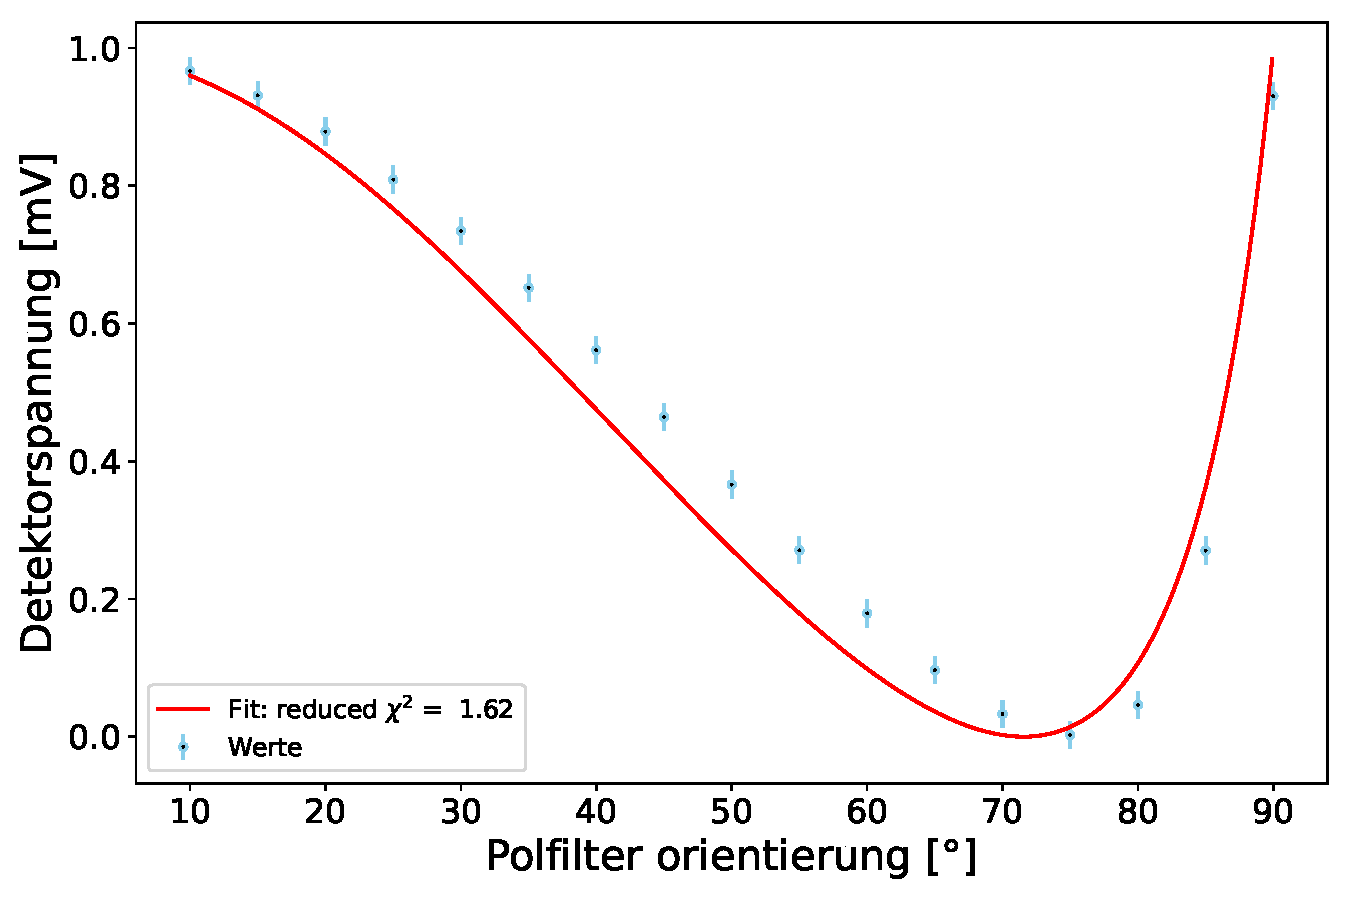
\includegraphics[width= 0.65 \textwidth]{Fits/Rp_Rs_Si_Fit.pdf} 
	\caption{Rp Rs Si, Fit} 
 	\label{fig:Rp Rs Si, Fit} 
\end{figure}
 
\begin{table}[ht] 
	\centering 
	\caption{Rp Rs Si, Fit Parameter Tabelle} 
	\label{tab: Rp Rs Si, Fit Parameter Tabelle}
	\begin{tabular}{|l|c|}
		\hline
		Parameter Name	&	Wert \\ \hline
		n	&	 3.733 $\pm$  0.0286\\ \hline
		kappa	&	-0.51709 $\pm$  0.105\\ \hline
	\end{tabular} 
\end{table}
 
\begin{table}[ht] 
	\centering 
	\caption{Rp Rs Si, Messwerte Tabelle} 
	\label{tab: Rp Rs Si, Messwerte Tabelle}
	\begin{tabular}{|c|c|}
		\hline
		Einfallswinkel $\Phi_i$ [°] 	&	 $\frac{R_p}{R_s}$\\ \hline
		90.0 $\pm$ 0.2 	&	 0.930 $\pm$ 0.005 \\ \hline
		85.0 $\pm$ 0.2 	&	 0.272 $\pm$ 0.002 \\ \hline
		80.0 $\pm$ 0.2 	&	 0.049 $\pm$ 0.002 \\ \hline
		75.0 $\pm$ 0.2 	&	 0.005 $\pm$ 0.003 \\ \hline
		70.0 $\pm$ 0.2 	&	 0.036 $\pm$ 0.003 \\ \hline
		65.0 $\pm$ 0.2 	&	 0.099 $\pm$ 0.003 \\ \hline
		60.0 $\pm$ 0.2 	&	 0.182 $\pm$ 0.003 \\ \hline
		55.0 $\pm$ 0.2 	&	 0.273 $\pm$ 0.004 \\ \hline
		50.0 $\pm$ 0.2 	&	 0.368 $\pm$ 0.004 \\ \hline
		45.0 $\pm$ 0.2 	&	 0.467 $\pm$ 0.005 \\ \hline
		40.0 $\pm$ 0.2 	&	 0.563 $\pm$ 0.005 \\ \hline
		35.0 $\pm$ 0.2 	&	 0.653 $\pm$ 0.006 \\ \hline
		30.0 $\pm$ 0.2 	&	 0.736 $\pm$ 0.006 \\ \hline
		25.0 $\pm$ 0.2 	&	 0.810 $\pm$ 0.007 \\ \hline
		20.0 $\pm$ 0.2 	&	 0.879 $\pm$ 0.007 \\ \hline
		15.0 $\pm$ 0.2 	&	 0.932 $\pm$ 0.007 \\ \hline
		10.0 $\pm$ 0.2 	&	 0.967 $\pm$ 0.008 \\ \hline
	\end{tabular} 
\end{table}
 
